\chapter{Adatbázisfüggvények}
\thispagestyle{empty}

Adatbázisfüggvények segítségével számításokat
végezhetünk az adattábla értékeivel egy dinamikusan
változtatható keresési tartomány feltételei alapján. Az
irányított szűrőhöz hasonlóan e tartomány egy
sorának cellái között ÉS logikai kapcsolat lesz, a sorok
között pedig VAGY. Minden adatbázisfüggvénynek három
argumentuma van: \textbf{adatbázis}, \textbf{adatbázismező}
és \textbf{keresési feltétel}.

Az első magát az adattáblát adja meg. Az irányított
szűrő tulajdonságait bemutató példánál ez az A1:E17
tartomány (\ref{SzűrésEredmények} ábra).

A \textbf{keresési feltétel} a feltételeket tartalmazó
cellatartomány. \Aref{SzűrésEredmények} ábrán a A22:E24.
Ebben a tartományban csak akkor használhatunk reguláris
kifejezéseket ha bekapcsoljuk az
\textbf{Eszközök --  Beállítások --  OpenOffice.org Calc --
Számítás} panelen a \textbf{Reguláris kifejezések
engedélyezése képletekben} kapcsolót.

Az \textbf{adatbázismező} annak az oszlopnak a sorszáma az
adattáblán belül, amelyikben a függvény működni fog. A 0
értékkel megadhatjuk a teljes adattartományt. Mezőnevet is
megadhatunk idézőjelek közé írva.


\Aref{AdatbázisFüggvények} táblázat a gyakrabban használt
adatbázisfüggvényeket mutatja.

\begin{table}[!h]
\begin{center}
\caption{Gyakrabban használt adatbázisfüggvények}\label{AdatbázisFüggvények}
\begin{tabular}{|m{2.5cm}|m{8cm}|}
\hline
AB.SUM &
A keresési feltételeknek megfelelő cellák összegét
számítja ki.\\ \hline
AB.MAX &
A keresési feltételeknek megfelelő cellák közül a
legnagyobb értékét adja vissza.\\ \hline
AB.MIN &
A keresési feltételeknek megfelelő cellák közül a
legkisebb értékét adja vissza.\\ \hline
AB.ÁTLAG &
A keresési feltételeknek megfelelő cellák átlagát
számítja ki.\\ \hline
AB.DARAB &
Megszámolja a számokat tartalmazó rekordokat az adattáblában,
amelyek megfelelnek a keresési feltételeknek.\\ \hline
AB.DARAB2 &
Megszámolja a számokat vagy szöveget tartalmazó (azaz nem üres) 
rekordokat az adattáblában, amelyek megfelelnek a keresési
feltételeknek.\\ \hline
\end{tabular}
\end{center}
\end{table}

\clearpage
\section{26. feladat}
{\itshape
Számítsuk ki adatbázisfüggvények felhasználásával \aref{IrányítottSzűrő} 
ábrán látható feltételeknek megfelelő rekordok:}

{\itshape
a) darabszámát}

{\itshape
b) készletszámok összegét}

{\itshape
c) a legnagyobb beszerzési árat }

{\itshape
d) a legkisebb beszerzési árat}

{\itshape
e) a beszerzési árak átlagát}

{\itshape
Módosítsuk a keresési feltételeket, hogy a K betűvel
kezdődő, 10~000~Ft-nál kisebb beszerzési árú
 rekordokat határozza meg.}

A szűrő kikapcsolása után másoljuk az A1:E24 tartományt
egy üres munkalapra. A Reguláris kifejezések engedélyezése
képletekben kapcsolót a Beállítások ablakban kapcsoljuk be.
Az A26:A30 tartományba írjuk \aref{26-feladat} ábrán látható
tartalmakat és adatbázisfüggvények segítségével
számítsuk ki a C26:C30 tartomány celláit. A rekordok
számának meghatározásánál használhatjuk az AB.DARAB
függvényt. Olyan mezőt válasszunk második argumentumnak,
amelyiket az adattábla módosításánál is mindenképp
kitöltünk. Esetünkben ilyen lehet az első, a Kód mező.

\begin{figure}[!h]
\begin{center}
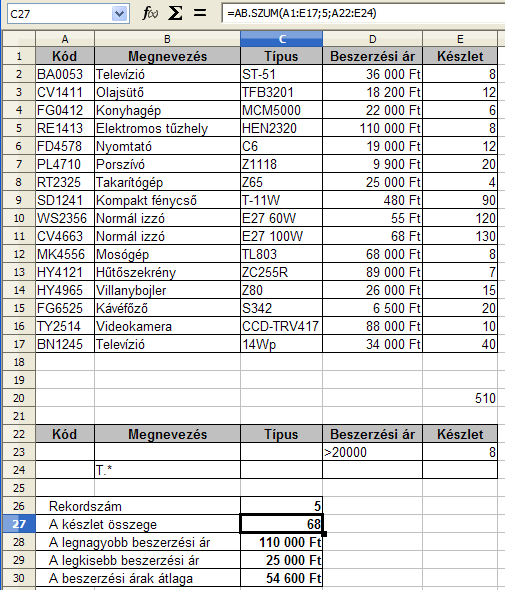
\includegraphics[width=12.36cm]{oocalcv2-img120.png}
\caption{26. feladat}\label{26-feladat}
\end{center}
\end{figure}

A készlet összegének kiszámításának képletét látjuk
\aref{26-feladat} ábrán. A további három függvény argumentuma ugyanaz
lesz: \textsf{\textbf{\textcolor{black}{(A1:E17;4;A22:E24)}}}, a
használt függvények pedig AB.MAX, AB.MIN és AB.ÁTLAG. Az első
két eredményt leellenőrizhetjük, összehasonlítva az
Irányított szűrő példájában kapottakkal. A RÉSZÖSSZEG
függvény ott ugyanúgy a készletszámok összegét
határozta meg, ugyanazokkal a keresési feltételekkel.

Módosítsuk a keresési feltételeket, és az
adatbázisfüggvények az új feltételeknek megfelelő
rekordok alapján határozzák meg az értékeket (\ref{26-feladatEredmény} ábra).

\begin{figure}[!h]
\begin{center}
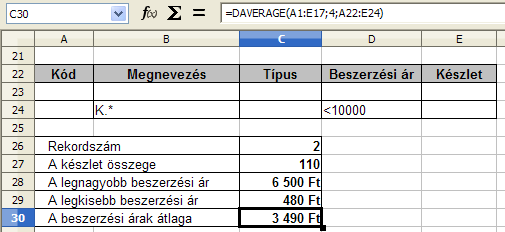
\includegraphics[width=12.36cm]{oocalcv2-img121.png}
\caption{26. feladat --  eredmény}\label{26-feladatEredmény}
\end{center}
\end{figure}

Az ebben a fejezetben tárgyalt függvények \aref{13-fejezetFüggvények}
táblázatban láthatóak.

\begin{table}[!h]
\begin{center}
\caption{A fejezetben tárgyalt függvények}\label{13-fejezetFüggvények}
\begin{tabular}{|m{3cm}|m{8cm}|m{3cm}|}
\hline
\multicolumn{1}{|c|}{\textbf{A függvény}}&
\multicolumn{1}{c|}{\textbf{Funkciója}}&
\multicolumn{1}{c|}{\textbf{A függvény}} \\
\multicolumn{1}{|c|}{\textbf{neve}} & &
\multicolumn{1}{c|}{\textbf{angol neve}} \\
\hline
AB.SZUM & A keresési feltételeknek megfelelő cellák összegét
számítja ki. & DSUM\\ \hline
AB.MAX & A keresési feltételeknek megfelelő cellák közül a
legnagyobb értékét adja vissza. & DMAX\\ \hline
AB.MIN & A keresési feltételeknek megfelelő cellák közül a
legkisebb értékét adja vissza. & DMIN\\ \hline
AB.ÁTLAG & A keresési feltételeknek megfelelő cellák átlagát
számítja ki. & DAVERAGE\\ \hline
AB.DARAB & Megszámolja a számokat tartalmazó rekordokat az adattáblában,
amelyek megfelelnek a keresési feltételeknek. & DCOUNT\\ \hline
AB.DARAB2 & Megszámolja a számokat vagy szöveget tartalmazó (azaz nem üres) rekordokat az
adattáblában, amelyek megfelelnek a keresési feltételeknek. &
DCOUNTA\\ \hline
\end{tabular}
\end{center}
\end{table}

